\chapter{Software Requirements Specification}
\label{chap:reqs}

\section{User Interactions and System Actors}
The FORGE system interacts with three primary classes of actors:
\begin{enumerate}
    \item \textbf{Primary Actor (Player):} Navigates the dungeon, engages in melee combat, evades enemy projectiles via dodge rolls, collects health pickups, avoids traps, and transitions through floor portals.
    \item \textbf{Secondary Actor (Game Balance Evaluator / Supervisor):} Monitors live telemetry via the Defense Overlay HUD, toggles between Adaptive PPO mode and Static Baseline mode, manually overrides difficulty parameters via sliders, and inspects exported session logs.
    \item \textbf{Automated System Actor (GitHub Actions CI Runner):} Executes automated headless test scripts, parses exit codes, and asserts topological solvability across randomized seeds.
\end{enumerate}

\section{Use Case Diagram}
Figure~\ref{fig:use_case_diagram} depicts the core use cases and actor associations within Project FORGE.

\begin{figure}[!htbp]
\centering
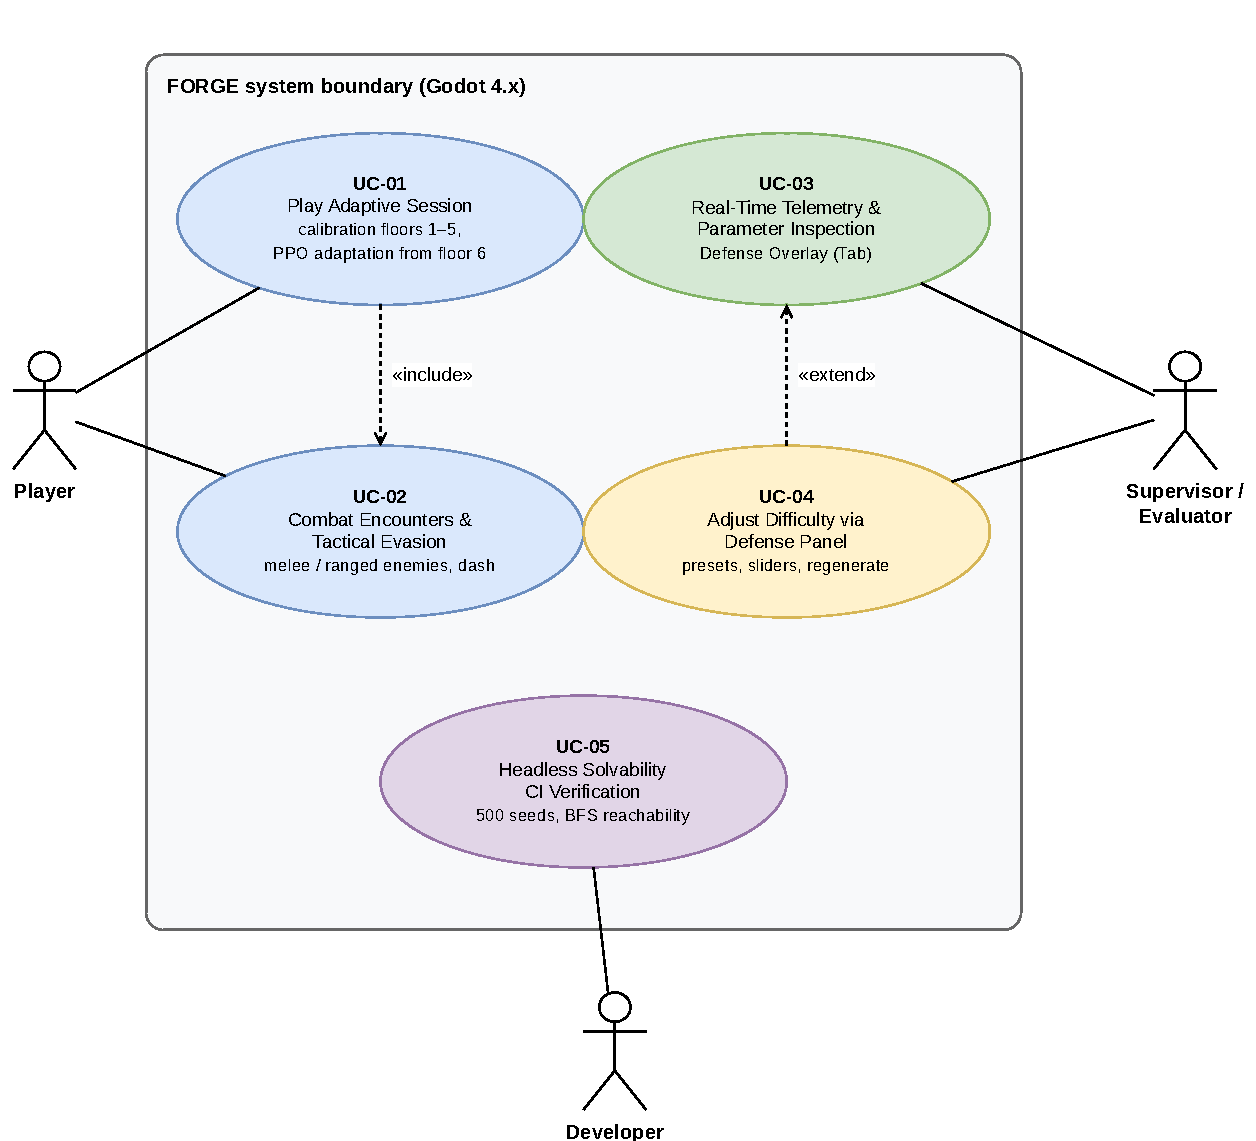
\includegraphics[width=0.95\textwidth]{ThesisFigs/fig_4_2_use_case}
\caption{Unified Use Case Diagram for Project FORGE}
\label{fig:use_case_diagram}
\end{figure}

\section{Detailed Use Cases}

\subsection{UC-01: Play Adaptive Session with Cold-Start Calibration}
\begin{itemize}
    \item \textbf{Actors:} Player (Primary), PPO Generator (System).
    \item \textbf{Preconditions:} Game is launched; player selects ``Start Game'' from the main menu; \texttt{policy\_weights.json} exists or heuristic fallback is ready.
    \item \textbf{Trigger:} Player initiates a new dungeon run.
    \item \textbf{Main Scenario:}
    \begin{enumerate}
        \item System loads Floor 1 in Cold-Start mode with baseline difficulty parameters ($\vec{E}_1, \vec{M}_1$).
        \item Player traverses rooms, defeats adversaries, and reaches the exit portal.
        \item \texttt{TelemetryLogger} records clearing time, damage ratio, and deaths.
        \item Steps 1--3 repeat through Floor 5 with escalating parameter tiers.
        \item At Floor 5 exit, system computes $CR_0 = \sum w_i \cdot \text{Score}_i / \sum w_i$ ($\vec{w} = [1.0, 1.5, 2.0, 2.5, 3.0]$).
        \item System builds the initial PPO observation $s_0$ from the same weighted calibration records, expressed on the policy's training scales (Equation~\ref{eq:s0_seed}), and predicts action $a_0$; $CR_0$ is shown to the player and evaluator as a summary.
        \item Floor 6 loads with personalized parameters; closed-loop PPO adaptation governs subsequent floors.
    \end{enumerate}
    \item \textbf{Alternative Path:} If the player dies, the death is recorded in telemetry and the player respawns in the start room of the current floor after 1.2\,s; cleared rooms stay cleared and difficulty parameters are unchanged until the floor is exited.
    \item \textbf{Postconditions:} One row per floor written to the SQLite database \texttt{user://forge\_telemetry.db} (JSON fallback \texttt{user://session\_telemetry.json} if the SQLite plugin is missing).
\end{itemize}

\subsection{UC-02: Combat Encounters and Tactical Evasion}
\begin{itemize}
    \item \textbf{Actors:} Player and the five enemy archetypes (Melee Crawler, Ranged Pyromancer, Heavy Brute, Agile Skirmisher, Swarmer; Table~\ref{tab:archetypes}). The steps below show the Crawler and Pyromancer; the other three follow the same pattern with their own telegraphs.
    \item \textbf{Preconditions:} Player enters a non-cleared room containing active enemies.
    \item \textbf{Main Scenario:}
    \begin{enumerate}
        \item Melee Crawlers detect player within aggro radius and initiate pursuit (default $125$\,px/s, PPO-controlled).
        \item Ranged Pyromancers hold a standoff distance ($140$--$280$\,px) and initiate $0.5$\,s telegraph tell.
        \item Pyromancers launch a fireball projectile along the direction to the player at the moment the telegraph ends (no lead prediction).
        \item Player executes Spacebar dodge roll ($0.2$\,s dash), gaining $0.26$\,s of invulnerability to evade the projectile.
        \item Player delivers sword strike to enemy hitbox; system computes damage, triggers camera shake (decay rate $3.6$\,s$^{-1}$), and pops yellow floating damage text.
        \item Enemies defeated; doors unlock. Health pickups were placed when the room was generated: a combat room holds a potion with probability $1 - \text{resource scarcity}$.
    \end{enumerate}
    \item \textbf{Postconditions:} Combat damage dealt and received logged by \texttt{TelemetryLogger}.
\end{itemize}

\subsection{UC-03: Real-Time Telemetry and Defense Inspection}
\begin{itemize}
    \item \textbf{Actors:} Game Evaluator / Supervisor.
    \item \textbf{Preconditions:} Game is actively running in gameplay state.
    \item \textbf{Trigger:} Evaluator presses the \texttt{Tab} key.
    \item \textbf{Main Scenario:}
    \begin{enumerate}
        \item System renders the semi-transparent Defense Telemetry Overlay HUD.
        \item HUD displays current floor index, active mode (Adaptive vs. Static), cold-start status, and raw observation signals ($s_t$).
        \item Displays live sliders showing current enemy health, damage, speed, aggro radius, hazard density, and room count.
        \item Evaluator adjusts a slider manually; system applies the override dynamically to the current floor.
    \end{enumerate}
    \item \textbf{Postconditions:} Parameter overrides reflected in real-time enemy behavior.
\end{itemize}

\subsection{UC-04: Give Consent and Rate a Floor (new for Final-1)}
\begin{itemize}
    \item \textbf{Actors:} Player (Primary), Telemetry Logger (System).
    \item \textbf{Preconditions:} Playtest or dev build is running.
    \item \textbf{Main Scenario:}
    \begin{enumerate}
        \item The consent screen explains what is recorded and asks whether the session may be used for research (currently at first launch; to be moved after the Play button, as the supervisor asked on 18 Nov 2026). The choice can be changed later under Main Menu $\rightarrow$ Data \& Privacy.
        \item After each finished floor, if the player consented, the game pauses and asks ``How hard did that floor feel?'' on a 1--5 scale (keys 1--5, Esc skips).
        \item The rating is stored in \texttt{floors.perceived\_difficulty}; a skipped rating is stored as NULL.
    \end{enumerate}
    \item \textbf{Alternative Path:} If the player declines, floors are still logged locally with \texttt{consent = 0}, no rating is asked, and the session is left out of all analysis.
    \item \textbf{Postconditions:} The \texttt{sessions.consent} flag and per-floor ratings are in \texttt{forge\_telemetry.db}.
\end{itemize}

\section{Functional Requirements}

\subsection{Module 1: Telemetry and Behavioral Profiling}
\begin{itemize}
    \item \textbf{FR-01 (Session Telemetry Collection):} The system shall capture room clearing duration, player damage received, damage dealt to enemies, death events, and potion pickups, logging events at 60\,FPS without frame latency.
    \item \textbf{FR-02 (Cold-Start Weighted Calibration):} The system shall enforce a 5-floor calibration sequence calculating an Initial Combat Rating ($CR_0 \in [10, 95]$) using non-uniform weights $\vec{w} = [1.0, 1.5, 2.0, 2.5, 3.0]$ across pace, survival, and damage execution.
    \item \textbf{FR-03 (SQLite Telemetry Persistence):} The system shall write one row per finished floor (outcomes, all eight settings, archetype mix, observation and action vectors, frame times, rating) to \texttt{user://forge\_telemetry.db}, and fall back to \texttt{user://session\_telemetry.json} if the SQLite plugin is missing.
    \item \textbf{FR-11 (Consent):} The system shall ask for research consent and store it per session; non-consented sessions shall be excluded from analysis.
    \item \textbf{FR-12 (Floor Rating):} For consented players the system shall ask for a 1--5 perceived-difficulty rating after each floor, which the player may skip.
\end{itemize}

\subsection{Module 2: Reinforcement Learning and Difficulty Policy}
\begin{itemize}
    \item \textbf{FR-04 (PPO Action Inference):} The system shall pass an 8-dimensional normalized observation vector ($s_t$) through an embedded MLP with two hidden layers in GDScript, producing an 8-dimensional continuous action vector ($a_t \in [-1, 1]^8$). A legacy 7-output policy file shall still be accepted.
    \item \textbf{FR-05 (Heuristic Fallback Autonomy):} If \texttt{policy\_weights.json} is missing or corrupted, the system shall engage a deterministic heuristic policy that adjusts parameters from a linear performance signal (clearing time, deaths, damage taken) without raising unhandled exceptions.
\end{itemize}

\subsection{Module 3: Dungeon Layout and Encounter Synthesis}
\begin{itemize}
    \item \textbf{FR-06 (Topological Connectivity):} The system shall generate connected room layouts (every room is attached to a previously placed room through a matching door pair), and the CI harness shall verify with a breadth-first search over the door graph that the exit room is reachable from the start room.
    \item \textbf{FR-07 (Parameter Denormalization):} The system shall map normalized PPO actions ($[-1, 1]$) into bounded game engine ranges: enemy health $[20, 120]$\,HP, enemy damage $[5, 50]$, enemy speed $[60, 220]$\,px/s, aggro radius $[100, 450]$\,px, hazard density $[0.05, 0.80]$, resource scarcity $[0.10, 0.90]$, room count $[5, 9]$, and archetype complexity $c = (a_7+1)/2 \in [0,1]$, which sets the enemy mix (Equation~\ref{eq:mix}).
    \item \textbf{FR-14 (BSP Baseline, planned):} The system shall offer a non-adaptive BSP layout generator that outputs the same room data as the FORGE generator, selectable as \texttt{generator\_mode = bsp}, and record the generator used in telemetry.
\end{itemize}

\subsection{Module 4: Core Gameplay and Combat}
\begin{itemize}
    \item \textbf{FR-08 (Multi-Archetype Enemy Combat):} The system shall spawn five enemy archetypes (Melee Crawler, Ranged Pyromancer, Heavy Brute, Agile Skirmisher, Swarmer), each with a telegraphed attack, sampled per spawn slot from the current archetype mix.
    \item \textbf{FR-09 (Player Dodge Roll):} The system shall execute an evasive dash on Spacebar input, lasting $0.2$\,s and granting $0.26$\,s of invulnerability, with a $1.0$\,s cooldown timer.
    \item \textbf{FR-10 (Static Roguelike Baseline Toggle):} The system shall provide an in-engine toggle disabling PPO adaptation and scaling enemy health and damage by a fixed $+8\%$ per floor.
\end{itemize}

\subsection{Module 5: Judge, Player Model and Explanations (offline)}
\begin{itemize}
    \item \textbf{FR-13 (Learned Judge):} The system shall provide a Judge trained from telemetry that predicts a floor's difficulty on $[0,1]$ from its settings and the previous floor's results, report MAE against the hand-weighted formula, and produce a per-floor SHAP explanation (Design Insight Report).
    \item \textbf{FR-15 (Player Model and Calibrated Simulator, planned):} The system shall provide a player model (MLP1) trained on real telemetry that predicts a player's time, deaths and damage for a given configuration, and a training environment that uses it in place of the hand-written simulator.
    \item \textbf{FR-16 (Policy SHAP, planned):} The system shall compute, for a given observation, how much each of the 8 inputs pushed each of the 8 policy outputs up or down.
    \item \textbf{FR-17 (In-game explanation, FYP-2):} The Defense Overlay shall show Judge and Policy explanations for the current floor.
\end{itemize}

\section{Non-Functional Requirements}

\subsection{Reliability and Fault Tolerance}
\begin{itemize}
    \item \textbf{NFR-01 (Zero-Crash Fallback):} The system shall gracefully degrade to the heuristic fallback policy upon missing or malformed JSON weights, maintaining continuous gameplay without crashing.
    \item \textbf{NFR-02 (Solvability Integrity):} The dungeon generator shall produce layouts in which every room is reachable from the start room, for every room count the game can request (3--9).
\end{itemize}

\subsection{Usability and Visual Polish}
\begin{itemize}
    \item \textbf{NFR-03 (Visual Feedback \& Juice):} Player and enemy damage events shall trigger trauma camera shake that settles within $0.3$\,s ($\le 1/3.6$\,s even at maximum trauma; about $0.12$\,s for a single hit) and spawn color-coded floating text numbers (yellow for enemy hit, red for player hurt, green for healing).
    \item \textbf{NFR-04 (Combat Telegraphing):} Ranged projectile attacks shall display a minimum $0.5$\,s visual tell prior to launch to allow human reaction.
\end{itemize}

\subsection{Performance and Latency}
\begin{itemize}
    \item \textbf{NFR-05 (Rendering Frame Rate):} The game engine shall maintain a stable $\ge 60$\,FPS rendering rate at the $1280\times720$ project resolution, with frame delta not exceeding $16.6$\,ms.
    \item \textbf{NFR-06 (Neural Inference Latency):} The in-engine pure-GDScript neural network forward pass shall compute action predictions with a median below $1.0$\,ms per invocation.
\end{itemize}

\subsection{Security and Data Privacy}
\begin{itemize}
    \item \textbf{NFR-07 (Privacy by Design):} The telemetry system shall collect no directly identifying data (no names, emails, IP addresses or device serials), use only a random pseudonymous \texttt{install\_id}, contain no network code, and use only consented sessions for analysis.
\end{itemize}

\subsection{Maintainability and Portability}
\begin{itemize}
    \item \textbf{NFR-08 (Maintainability):} Every push shall pass ruff lint, the \texttt{pytest} suite and the headless GDScript tests in CI.
    \item \textbf{NFR-09 (Portability):} A Windows build shall be exportable from the CI export preset without manual steps.
\end{itemize}

\section{Requirement Priorities and Final-1 Status}
Table~\ref{tab:req_priority} gives every requirement a MoSCoW priority (Must, Should, Could) and its status. Requirements FR-11 to FR-17 and NFR-08 to NFR-09 are new for Final-1.

\begin{table}[!htbp]
\centering
\caption{Requirement Priorities and Status at Final-1}
\label{tab:req_priority}
\scriptsize
\begin{tabular}{p{0.08\textwidth}p{0.46\textwidth}p{0.10\textwidth}p{0.26\textwidth}}
\toprule
\textbf{ID} & \textbf{Requirement (short)} & \textbf{Priority} & \textbf{Status} \\
\midrule
FR-01 & Per-floor telemetry capture & Must & \stdone \\
FR-02 & Five-floor calibration and $CR_0$ & Must & \stdone \\
FR-03 & SQLite persistence with JSON fallback & Must & \stdone \\
FR-04 & 8-D PPO inference in GDScript & Must & \stdone \\
FR-05 & Heuristic fallback & Must & \stdone \\
FR-06 & Connected layouts, BFS-checked & Must & \stdone \\
FR-07 & Action denormalization and archetype mix & Must & \stdone \\
FR-08 & Five enemy archetypes & Must & \stdone \\
FR-09 & Dodge roll & Must & \stdone \\
FR-10 & Static $+8\%$ baseline & Must & \stdone \\
FR-11 & Consent screen & Must & \stdone{} (move after Play: \stplan) \\
FR-12 & 1--5 floor rating & Must & \stdone \\
FR-13 & Learned Judge with SHAP explanations (offline) & Must & \stdone{} (synthetic training) \\
FR-14 & BSP baseline generator & Must & \stplan \\
FR-15 & Player model MLP1 and calibrated simulator & Must & \stplan \\
FR-16 & Policy SHAP on the PPO actor & Should & \stplan \\
FR-17 & Judge and SHAP shown inside the game & Could & \stplan{} (FYP-2 Mid) \\
NFR-01 to NFR-04 & Fallback, solvability, feedback, telegraphs & Must & \stdone \\
NFR-05 & 60\,FPS & Must & Logged; \tofill{value} \\
NFR-06 & Inference median $<1$\,ms & Must & \tofill{re-measure} \\
NFR-07 & Privacy and consent & Must & \stdone{} (text corrected) \\
NFR-08 & Maintainability: lint and tests pass in CI on every push & Should & \stdone \\
NFR-09 & Portability: Windows build from CI export preset & Should & \stdone{} (Windows only) \\
\bottomrule
\end{tabular}
\end{table}

\section{Acceptance Criteria}
Table~\ref{tab:acceptance_criteria} defines the objective acceptance criteria used to verify requirements completion.

\begin{table}[!htbp]
\centering
\caption{Requirements Acceptance Criteria and Verification Protocol}
\label{tab:acceptance_criteria}
\small
\begin{tabular}{p{0.12\textwidth}p{0.32\textwidth}p{0.34\textwidth}p{0.14\textwidth}}
\toprule
\textbf{Req. ID} & \textbf{Acceptance Metric} & \textbf{Verification Protocol} & \textbf{Final-1 Status} \\
\midrule
FR-01 & Event Capture Precision & Scripted hits (20 taken, $3\times35$ dealt) appear exactly in the snapshot (TC-01, headless) & Passed (after fix DEF-05) \\
FR-02 & $CR_0$ and $s_0$ & $CR_0 \in [10, 95]$ matches hand-computed values; $s_0$ on training scales (TC-02, headless) & Passed (after fix DEF-06) \\
FR-03 & SQLite persistence & Rows written to the real SQLite extension; JSON fallback when missing (\texttt{test\_telemetry\_sqlite}, \texttt{test\_telemetry\_fallback}) & Passed \\
FR-04 & Inference Execution & Action vector strictly within $[-1, 1]^8$ & Passed \\
FR-05 & Heuristic Fallback & Game proceeds normally when weights deleted & Passed \\
FR-06 & Topological Connectivity & All rooms reachable by BFS, 500 seeds $\times$ room counts 3--9 & Passed (3,500/3,500) \\
FR-08 & Five archetypes & Each archetype spawns with its multipliers; mix follows $c$; a Swarmer slot gives 3 bodies (\texttt{test\_enemy\_archetypes}, \texttt{test\_archetype\_mix}, \texttt{test\_swarm\_room}) & Passed \\
FR-09 & Dash Invulnerability & Zero damage registered when hit during dash & Passed \\
FR-10 & Static Baseline Scaling & Exactly $+8\%$ stat increase per floor verified & Passed \\
FR-11/12 & Consent and rating & Rating shown only after consent; stored per floor (\texttt{test\_playtest\_flow}) & Passed \\
FR-13 & Learned Judge & Test MAE $\le 0.15$ and below the linear formula; SHAP values add up to the prediction (\texttt{test\_judge.py}) & Passed (synthetic data) \\
FR-14 & BSP baseline & 200 seeds $\times$ 4--10 rooms connected, exit reachable, no overlaps (\texttt{test\_bsp\_generator}, planned) & Planned \\
NFR-05 & Rendering Performance & p95 frame time $\le 16.6$\,ms from logged floors on a stated machine & \tofill{value from real floors} \\
NFR-06 & Inference Latency & Median forward pass $<1.0$\,ms (\texttt{benchmark\_inference.gd}) & Passed at Mid-1 (7-output policy); \tofill{re-run on shipped policy} \\
\bottomrule
\end{tabular}
\end{table}

\section{Requirements Traceability Matrix}
Table~\ref{tab:rtm} maps requirements to system architecture modules, design artifacts, code implementations, and verification test cases.

\begin{table}[!htbp]
\centering
\caption{Requirements Traceability Matrix (RTM)}
\label{tab:rtm}
\scriptsize
\begin{tabular}{p{0.10\textwidth}p{0.18\textwidth}p{0.20\textwidth}p{0.24\textwidth}p{0.16\textwidth}}
\toprule
\textbf{Req. ID} & \textbf{Module} & \textbf{Design Artifact} & \textbf{Implementation File} & \textbf{Test Case} \\
\midrule
FR-01 & Telemetry Engine & Activity Diagram Fig.~\ref{fig:activity_session} & \texttt{TelemetryLogger.gd} & TC-01 \\
FR-02 & Profiling Engine & Sequence Diagram Fig.~\ref{fig:seq_diagram} & \texttt{TelemetryLogger.gd} & TC-02 \\
FR-03 & Storage Subsystem & SQLite schema Table~\ref{tab:sqlite_schema}, Fig.~\ref{fig:erd} & \texttt{SqliteBackend.gd}, \texttt{schema.sql} & TC-11, TC-12 \\
FR-04 & RL Policy Engine & UML Class Diagram Fig.~\ref{fig:class_diagram} & \texttt{PPOPolicy.gd} & TC-03 \\
FR-05 & RL Policy Engine & Listing~\ref{lst:fallback} & \texttt{PPOPolicy.gd} & TC-04 \\
FR-06 & Dungeon Generator & Two-Stage Pipeline Fig.~\ref{fig:two_stage_detail} & \texttt{DungeonGenerator.gd} & TC-06 (CI Headless) \\
FR-07 & Encounter Adapter & Parameter Mapping Table~\ref{tab:param_ranges} & \texttt{DifficultyManager.gd} & TC-05 \\
FR-08 & Combat Engine & Table~\ref{tab:archetypes}, Fig.~\ref{fig:state_enemy} & \texttt{Enemy.gd}, \texttt{Room.gd}, \texttt{SlamShockwave.gd} & TC-07, TC-08, TC-13 \\
FR-09 & Player Controller & Player FSM & \texttt{Player.gd} & TC-09 \\
FR-10 & Evaluation HUD & UI Component Layout & \texttt{DefenseOverlay.gd} & TC-10 \\
FR-11/12 & Playtest UI & UC-04 & \texttt{ConsentScreen.gd}, \texttt{FloorRating.gd} & TC-14 \\
FR-13 & Judge (offline) & Section~\ref{sec:judge} & \texttt{ml\_spike/judge/} & TC-15 \\
FR-14 to FR-16 & Baseline, ML pipeline & Section~\ref{sec:revised_arch} & planned & planned \\
NFR-01 & RL Policy Engine & Heuristic Branch & \texttt{PPOPolicy.gd} & TC-04 \\
NFR-02 & Dungeon Generator & Solvability Verifier & \texttt{DungeonGenerator.gd} & TC-06 \\
NFR-05 & Graphics Engine & Frame-time columns & \texttt{TelemetryLogger.gd} & Logged per floor \\
NFR-06 & RL Policy Engine & Benchmark Routine & \texttt{PPOPolicy.gd} & TC-03 + benchmark \\
\bottomrule
\end{tabular}
\end{table}
